\documentclass{svproc}
\usepackage{graphicx}
\usepackage{booktabs}
\usepackage[margin=1in]{geometry}
\usepackage{float}
\usepackage{adjustbox}
\usepackage{amsmath}
\usepackage{cite}
\usepackage{orcidlink}

\begin{document}

\title{Model Performance Report}

\author{Simon Green\inst{1}, Abdulrahman Altahhan\inst{2}}

\institute{
    School of Computing, University of Leeds, UK \\
    \inst{1} MSc, Artificial Intelligence \orcidlink{0009-0000-3537-6890} \\
    \inst{2} Senior Teaching Fellow in Artificial Intelligence \orcidlink{0000-0003-1133-7744} \\
    \email{\{od21sg, a.altahhan\}@leeds.ac.uk}
}

\date{\today}

\maketitle

\begin{center}
  {\it Results are updated in realtime from the evaluations.}
\end{center}

%----------------------------------------------------------

\section{Results and Model Comparison}

This report presents the performance evaluation of four reinforcement learning models: GenTRPO, TRPOER, and TRPOR. These models are implemented using \textbf{Stable Baselines3} and utilize \textbf{mini-batch gradient descent} approach. We benchmark against TRPO and PPO \cite{schulman2017trustregionpolicyoptimization, schulman2017proximalpolicyoptimizationalgorithms}. The entropy calculations guiding the models are based on the entropy of each mini-batch.

%----------------------------------------------------------

\subsection{EnTRPO (Trust Region Policy Optimization Method with Entropy Regularization)}

The EnTRPO model extends TRPO by incorporating an entropy regularization term in the policy objective and adds a replay buffer with a specific 97.5\% reward buffer reset logic \cite{roostaie2021entrpotrustregionpolicy}. While we do not present evaluations for this model, we include it in the discussion since it was used to inform some of the design decisions for other models evaluated. In the paper, the author does not discuss whether the replay buffer is prioritized or not, nor could we find any implementation or results for this model.

%----------------------------------------------------------

\subsection{TRPOR (TRPO with Entropy Regularization)}

This model extends TRPO by introducing entropy regularization only in the policy objective. The entropy coefficient hyperparameter guides the degree of regularization, ensuring a balance between exploration and exploitation. The entropy guiding this model is computed at the batch level, dynamically adjusting policy updates. The policy objective with entropy regularization is as follows:

\begin{equation}
J(\theta) = \operatorname{E}_{s,\, a \sim \pi_{\theta_{\text{old}}}}
\left[
\frac{\pi_\theta(a \mid s)}{\pi_{\theta_{\text{old}}}(a \mid s)}\, A(s,a)
\right]
+ \beta\, \operatorname{E}_{s \sim \rho^\pi}
\left[
H\left(\pi_\theta(\cdot \mid s)\right)
\right]
\end{equation}

\noindent
where \(\theta\) is the current policy parameter vector, \(\theta_{\text{old}}\) is the previous policy parameter vector, \(\pi_\theta(a \mid s)\) and \(\pi_{\theta_{\text{old}}}(a \mid s)\) are the current and old policy probabilities, \(A(s,a)\) is the advantage function, \(\rho^\pi\) is the state distribution under the current policy, \(\beta\) is the entropy regularization coefficient, and \(H\left(\pi_\theta(\cdot \mid s)\right)\) is the entropy of the policy at state \(s\).

%----------------------------------------------------------


\subsection{TRPOER (TRPO with Entropy Regularized Experience Replay)}

This model extends TRPO by incorporating entropy-based experience replay along with an additional policy entropy regularization term. In TRPOER, a prioritized experience replay buffer is employed where experiences are sampled according to the entropy of the current mini-batch, modulated by a hyperparameter coefficient. This bidirectional adaptive sampling mechanism adjusts both the number and the direction of sampled experiences to optimize learning. The adaptive sampling function is formulated as follows:

\begin{equation}
S(H, \kappa) =
\begin{cases}
S_{\max}, & \text{if } \sigma(H) \geq \lvert \kappa \rvert, \quad \kappa \geq 0 \\
S_{\min}, & \text{if } \sigma(H) < \lvert \kappa \rvert, \quad \kappa \geq 0 \\
S_{\max}, & \text{if } \sigma(H) \leq \lvert \kappa \rvert, \quad \kappa < 0 \\
S_{\min}, & \text{if } \sigma(H) > \lvert \kappa \rvert, \quad \kappa < 0
\end{cases}
\end{equation}

\noindent where \( S(H, \kappa) \) represents the number of replay samples drawn based on entropy \( H \) of the mini-batch, and \( \kappa \) is the sampling coefficient acting as an adaptive cutoff threshold. The function \( \sigma(H) \) normalizes entropy into the range \( [0,1] \) using a sigmoid transformation:

\begin{equation}
\sigma(H) = \frac{1}{1 + e^{-H}}
\end{equation}

\noindent ensuring bounded entropy-driven prioritization. For \( \kappa > 0 \), sampling is triggered when the normalized entropy \( \sigma(H) \) {\it exceeds} the threshold \( \lvert \kappa \rvert \), whereas for \( \kappa < 0 \), sampling is triggered when \( \sigma(H) \) {\it falls below} the threshold. This bidirectional gating mechanism enables adaptive experience replay that dynamically adjusts to policy entropy variations during training.

The underlying hypothesis for TRPOER originates from previous experiments with modified EnTRPO variants (namely, EnTRPOLow and EnTRPOHigh). In those experiments, only the replay buffer was sampled, without directly incorporating an entropy term into the policy objective. Although these variants sometimes outperformed standard TRPO in certain environments, their performance was inconsistent. This observation motivated the development of an adaptive sampling strategy—controlled by the sampling coefficient \( \kappa \)—that dynamically adjusts the replay mechanism to achieve robust performance across diverse scenarios. We also observed that the EnTRPO model with Prioritized Experience Replay (PER) outperformed the EnTRPO without, hence motivating the use of prioritized experience replay in TRPOER.


%----------------------------------------------------------


\subsection{GenTRPO (Generative Experience Replay Trust Region Policy Optimization with Entropy Regularization)}

Quite a mouth full, we'll find a better name. The GenTRPO algorithm extends the Trust Region Policy Optimization with Entropy Regularization (TRPOER) framework \cite{schulman2017proximalpolicyoptimizationalgorithms,schulman2017trustregionpolicyoptimization} by incorporating a generative model to augment the experience replay buffer. The key idea is to leverage synthetic experiences generated by a forward dynamics model to complement real experiences, thereby improving exploration and sample efficiency \cite{pathak2017curiositydrivenexplorationselfsupervisedprediction}. 

In the GenTRPO framework, the experiences used for policy updates are sampled from a replay buffer. The sampling strategy ensures that half of the samples in each batch are real experiences collected from the environment, while the other half are generated by the forward dynamics model. This combination of real and synthetic data balances model fidelity with exploratory richness, enabling the policy to generalize effectively while maintaining stability during optimization.

The generative component of GenTRPO relies on a forward dynamics model inspired by the intrinsic curiosity module \cite{pathak2017curiositydrivenexplorationselfsupervisedprediction}. The forward dynamics model comprises an encoder and a dynamics predictor. The encoder maps raw states \( s \) into a compact latent space representation \( h(s) \), capturing the essential features of the environment. The dynamics predictor then takes the latent state \( h(s) \) and action \( a \) as input and predicts the next latent state \( h(s') \), effectively modeling the transition function \( P(s' | s, a) \). The error of this model, expressed as 

\begin{equation}
  \mathcal{F}(s, a, s', r) = \frac{1}{2} \left\| g(h(s), a) - h(s') \right\|^2
\end{equation}
\noindent
where \( g(h(s), a) \) is the predicted latent state, \( h(s') \) is the true latent state, and \( \| \cdot \| \) represents the Euclidean norm. This error quantifies how accurately the forward dynamics model predicts the latent state transitions. It is used to compute intrinsic motivation, encouraging the agent to explore transitions that are harder to predict, thereby fostering exploration  \cite{wang2024prioritizedgenerativereplay}.



%----------------------------------------------------------

\section{Model Performance Table}

The table below summarizes the models' performance in terms of mean and standard deviation of rewards, along with maximum and minimum rewards recorded during training. A higher mean reward suggests better overall performance, while lower standard deviation indicates increased stability.

\bigskip
\begin{center}
  \begin{tabular}{|l|p{3.2cm}|p{3.2cm}|p{3.2cm}|p{3.2cm}|}
\toprule
Environment & Pendulum-v1 & InvertedDoublePendulum-v5 & Ant-v5 & Humanoid-v5 \\
Model &  &  &  &  \\
\midrule \\ \hline
PPO & $\begin{array}{c} -0.02M \\ -207.56\mu \pm 118.01\sigma \\ 2892E, 10R \end{array}$ & $\begin{array}{c} 9359.93M \\ 1090.87\mu \pm 2910.66\sigma \\ 6965E, 10R \end{array}$ & $\begin{array}{c} 1173.61M \\ 515.51\mu \pm 326.48\sigma \\ 1895E, 10R \end{array}$ & $\begin{array}{c} N/A \end{array}$ \\ \\ \hline
TRPO & $\begin{array}{c} -0.20M \\ -141.97\mu \pm 115.55\sigma \\ 2600E, 10R \end{array}$ & $\begin{array}{c} 9359.78M \\ 7516.76\mu \pm 3879.62\sigma \\ 5767E, 10R \end{array}$ & $\begin{array}{c} 1960.61M \\ 1328.68\mu \pm 284.88\sigma \\ 1067E, 10R \end{array}$ & $\begin{array}{c} 1247.77M \\ 369.87\mu \pm 311.76\sigma \\ 9569E, 10R \end{array}$ \\ \\ \hline
TRPOR & $\begin{array}{c} -0.22M \\ -197.32\mu \pm 215.34\sigma \\ 4508E, 10R \end{array}$ & $\begin{array}{c} 9357.32M \\ 8045.50\mu \pm 2918.29\sigma \\ 9123E, 5R \end{array}$ & $\begin{array}{c} 3590.62M \\ 1662.87\mu \pm 1171.26\sigma \\ 1655E, 7R \end{array}$ & $\begin{array}{c} 1416.67M \\ 620.72\mu \pm 381.70\sigma \\ 9225E, 10R \end{array}$ \\ \\ \hline
trpoer & $\begin{array}{c} N/A \end{array}$ & $\begin{array}{c} N/A \end{array}$ & $\begin{array}{c} 1349.85M \\ 1349.85\mu \pm 0.00\sigma \\ 1882E, 1R \end{array}$ & $\begin{array}{c} N/A \end{array}$ \\ \\ \hline
\bottomrule \\ \hline
\end{tabular}

\end{center}
\bigskip

\section{Performance Analysis Through Plots}

The following plots visualize different aspects of model performance.

\subsection{Resampled Rewards and Outlier Removal}

\begin{figure}[H]
    \centering
    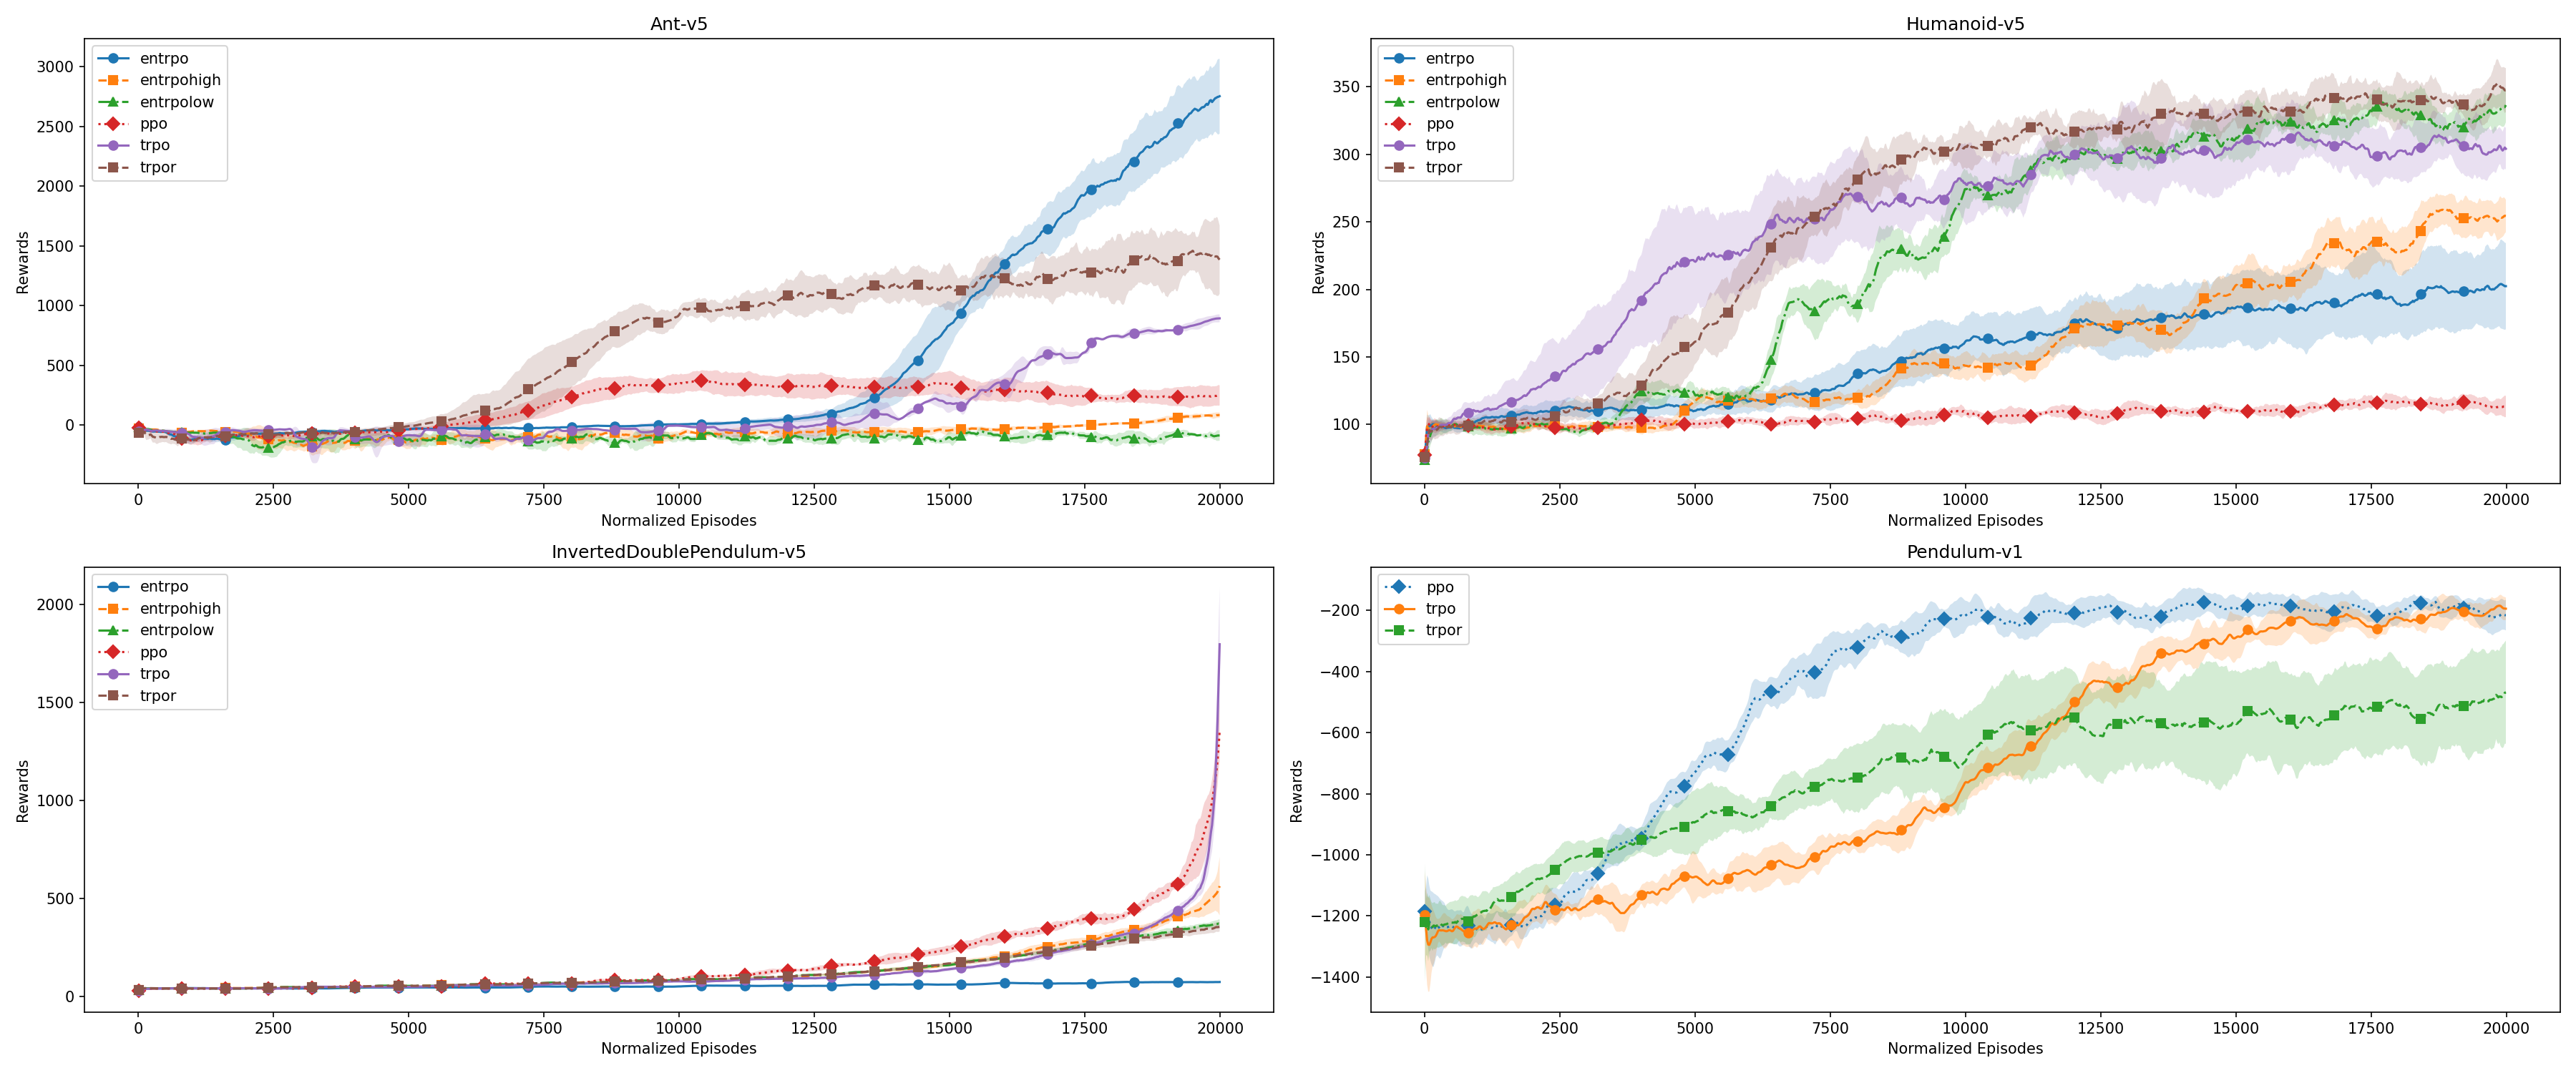
\includegraphics[width=0.8\textwidth]{.assets/resampled_outlier.png}
    \caption{Resampled Rewards with Outlier Removal}
\end{figure}

This plot presents reward distributions after applying smoothing and outlier removal techniques, filtering out misleading fluctuations.

\subsection{Learning Stability}

\begin{figure}[H]
    \centering
    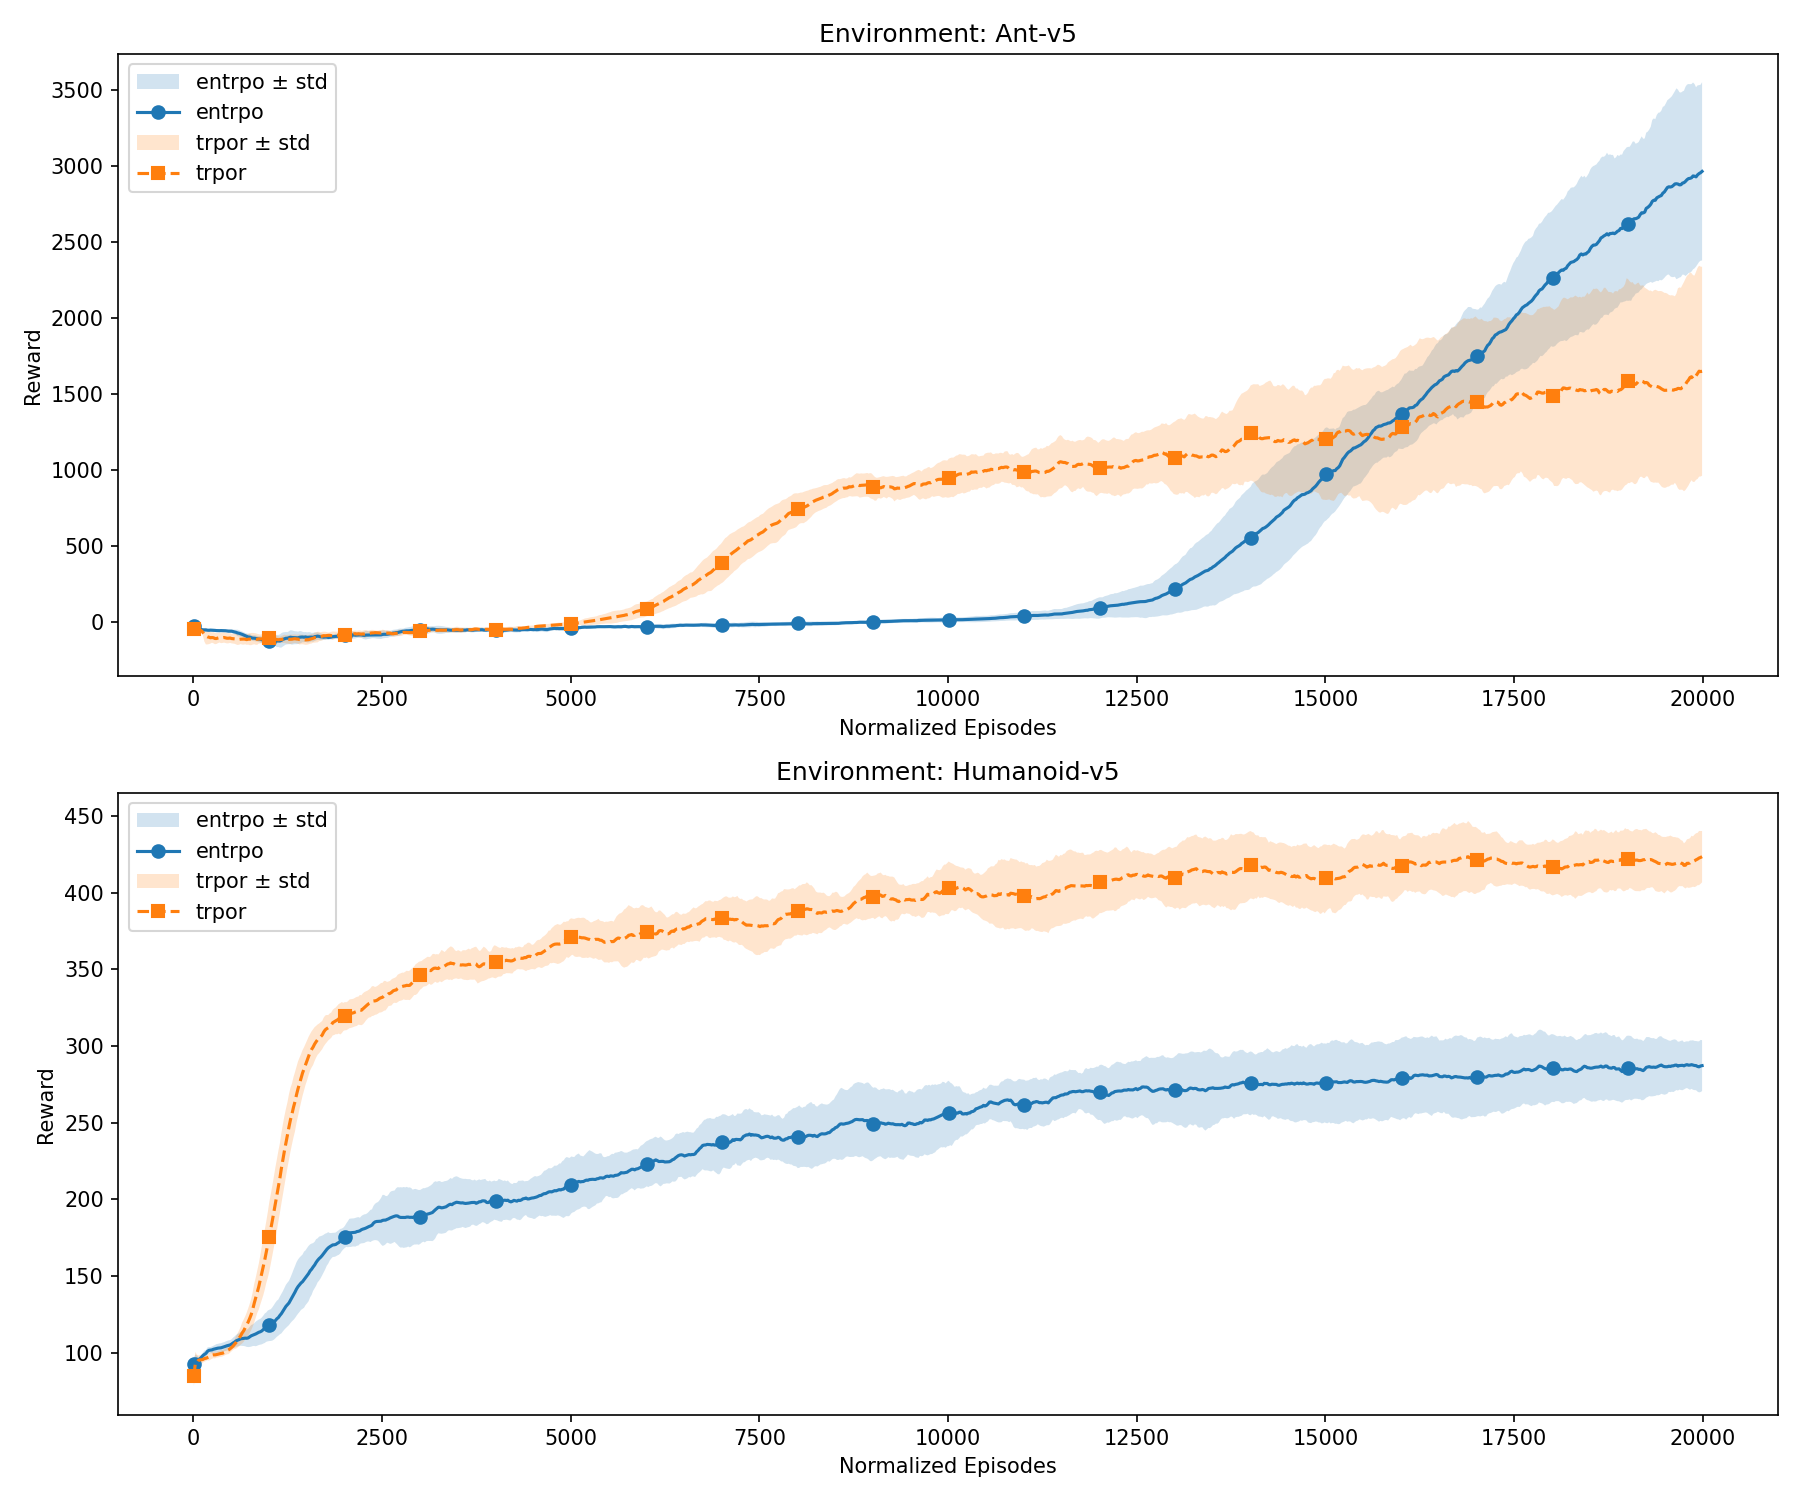
\includegraphics[width=0.8\textwidth]{.assets/learning_stability.png}
    \caption{Learning Stability for Different Models}
\end{figure}

Learning stability is evaluated based on the smoothness of the reward curve. A more stable learning process exhibits a steadily increasing reward trajectory, whereas high variance suggests instability due to sensitivity to hyperparameters.

\subsection{Learning Stability (Coefficient of Variation)}

\begin{figure}[H]
    \centering
    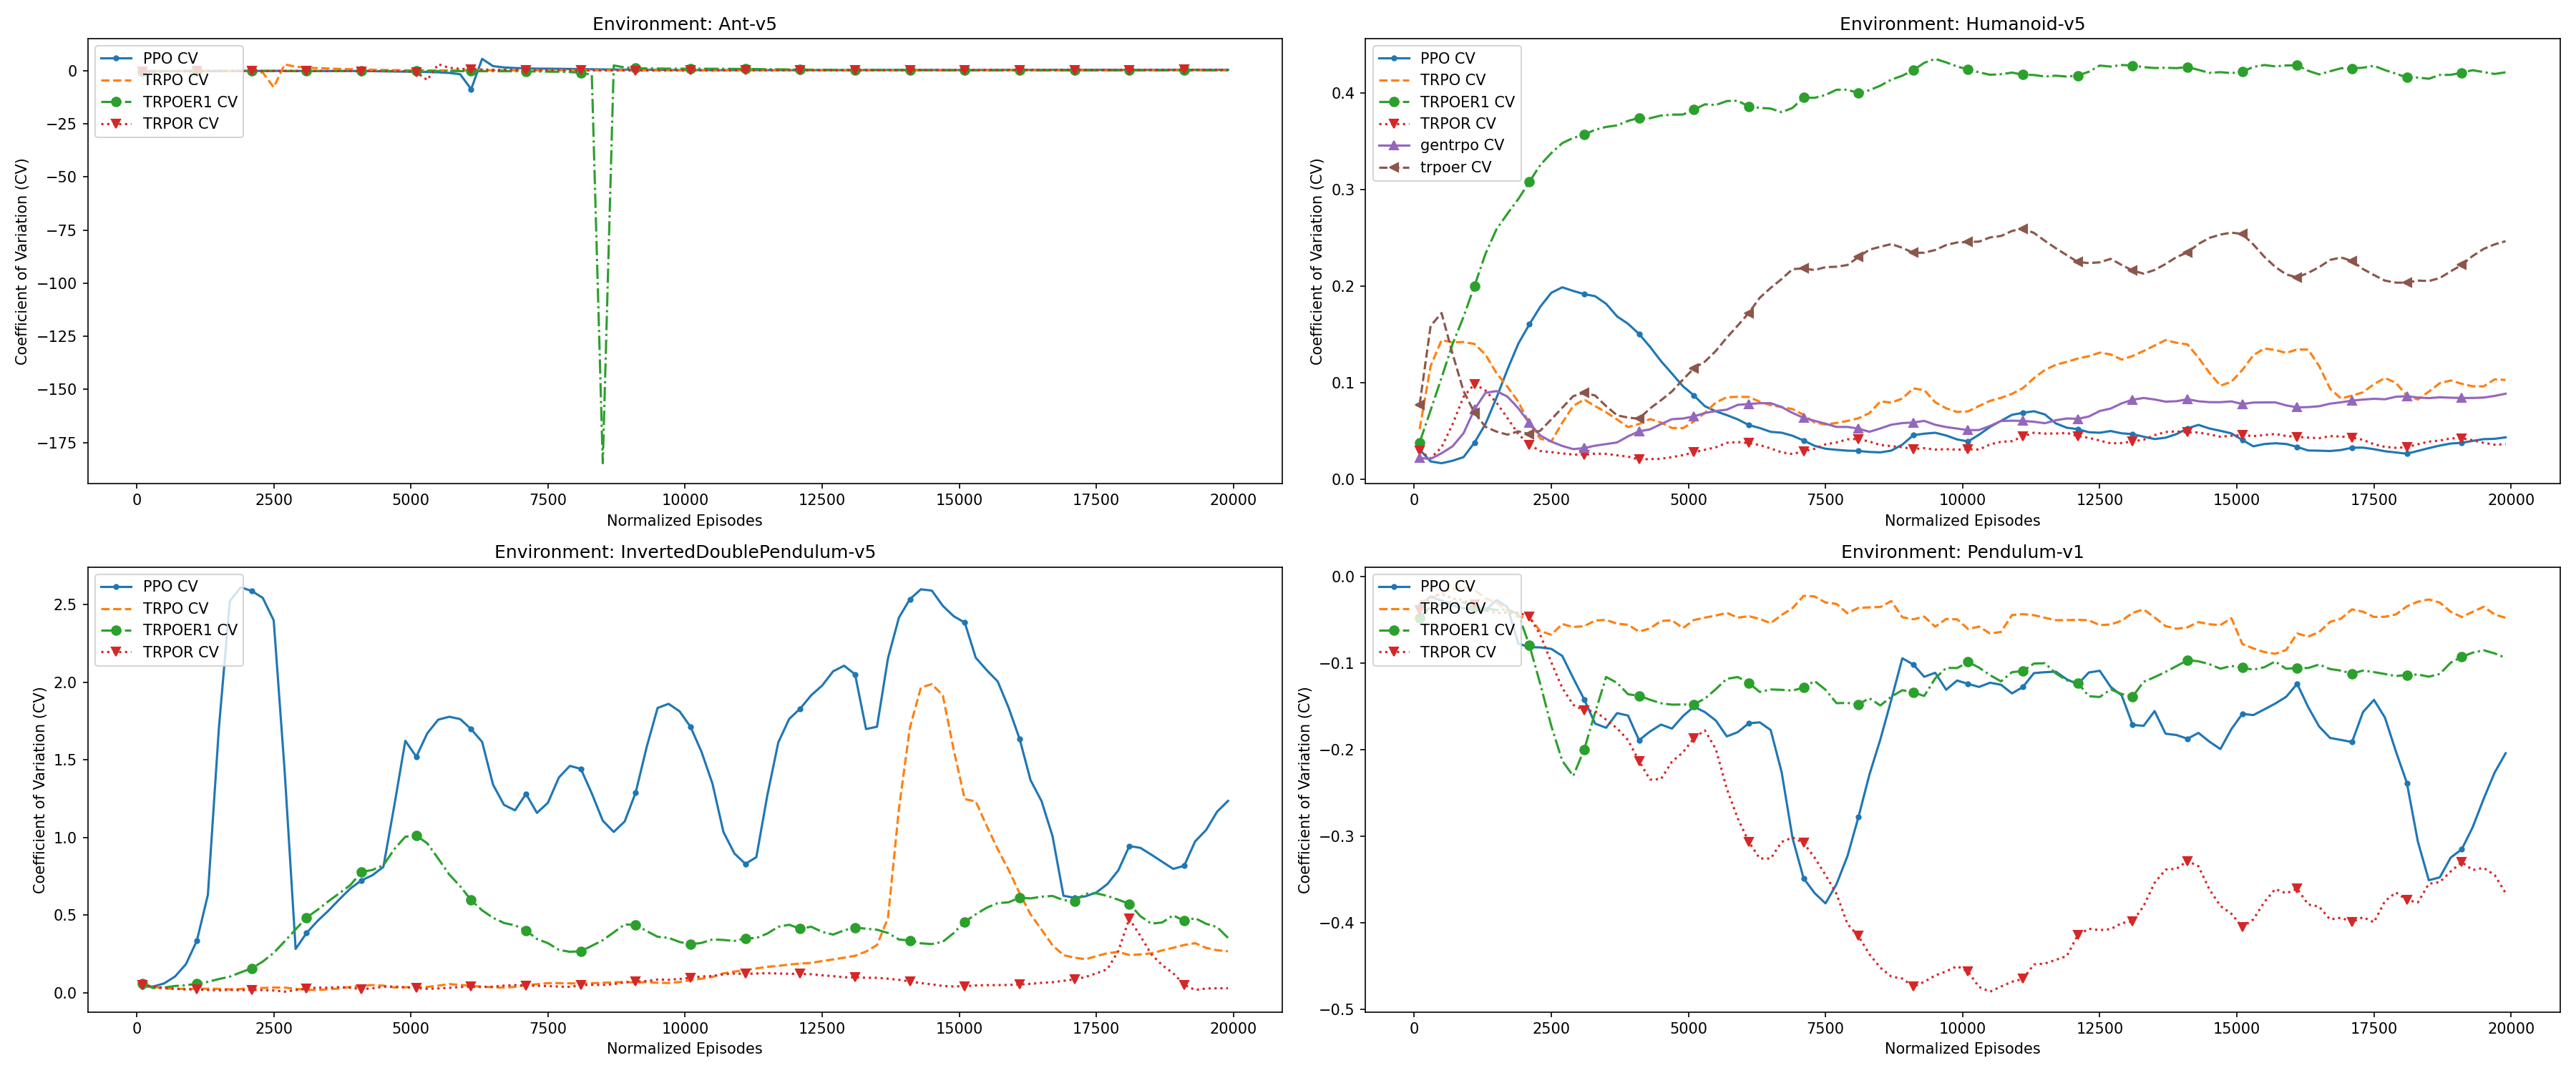
\includegraphics[width=0.8\textwidth]{.assets/learning_stability_cv.png}
    \caption{Learning Stability (Coefficient of Variation)}
\end{figure}

The coefficient of variation (CV) provides a normalized measure of stability. A lower CV signifies less volatile performance, whereas a higher CV indicates inconsistency due to randomness in training.

\subsection{Sample Efficiency}

\begin{figure}[H]
    \centering
    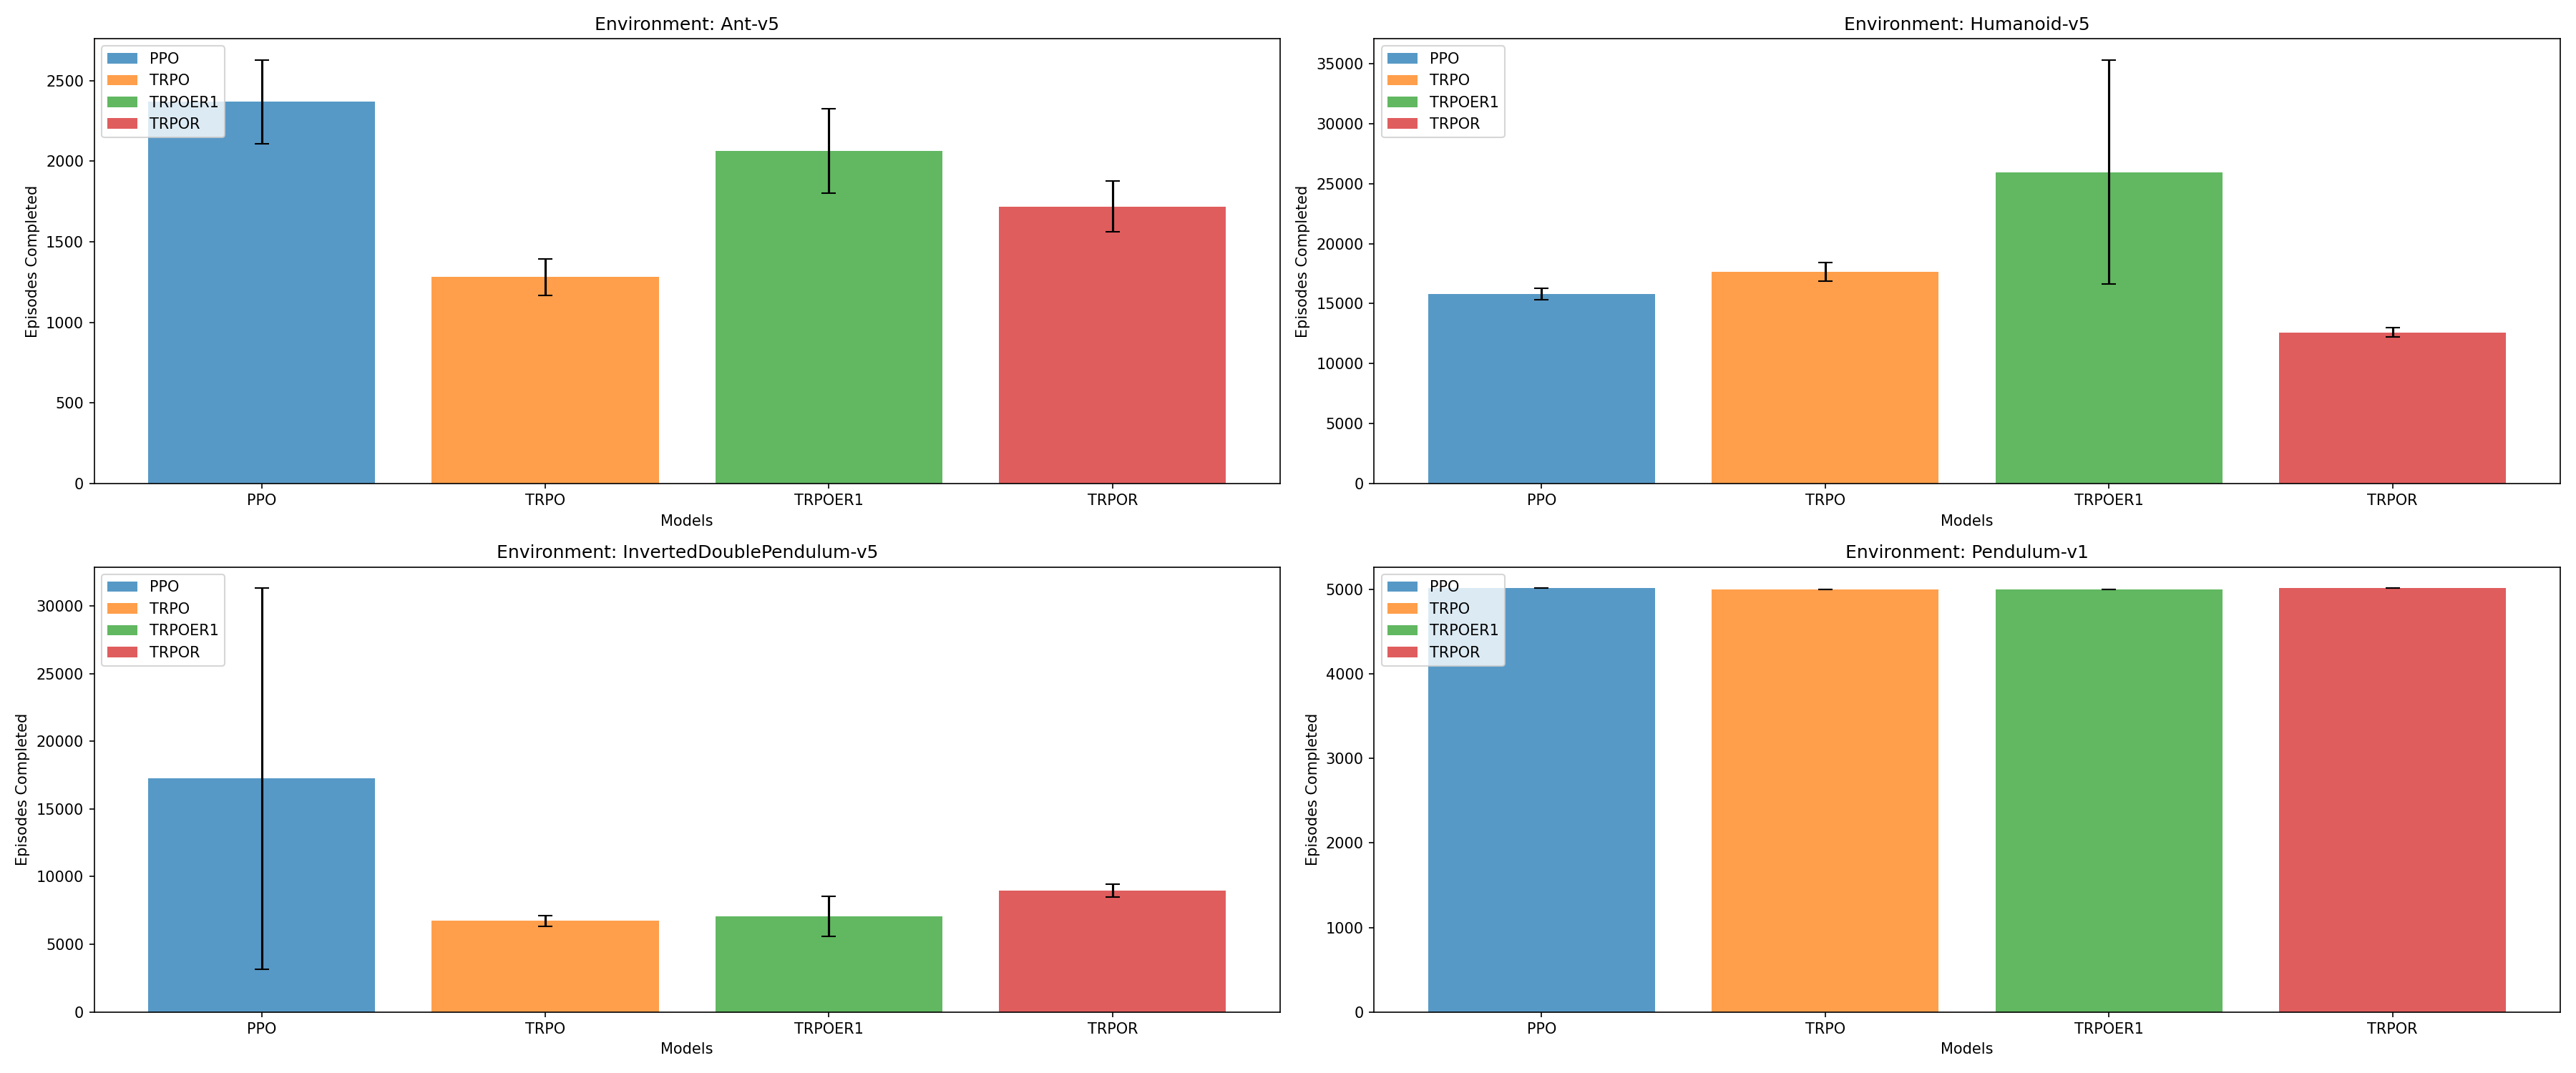
\includegraphics[width=0.8\textwidth]{.assets/sample_efficiency.png}
    \caption{Sample Efficiency Across Models}
\end{figure}

Sample efficiency measures how quickly a model improves with limited training episodes. Higher sample efficiency is desirable, especially in data-scarce scenarios.

\subsection{Combined Sample Efficiency Results}

\begin{figure}[H]
    \centering
    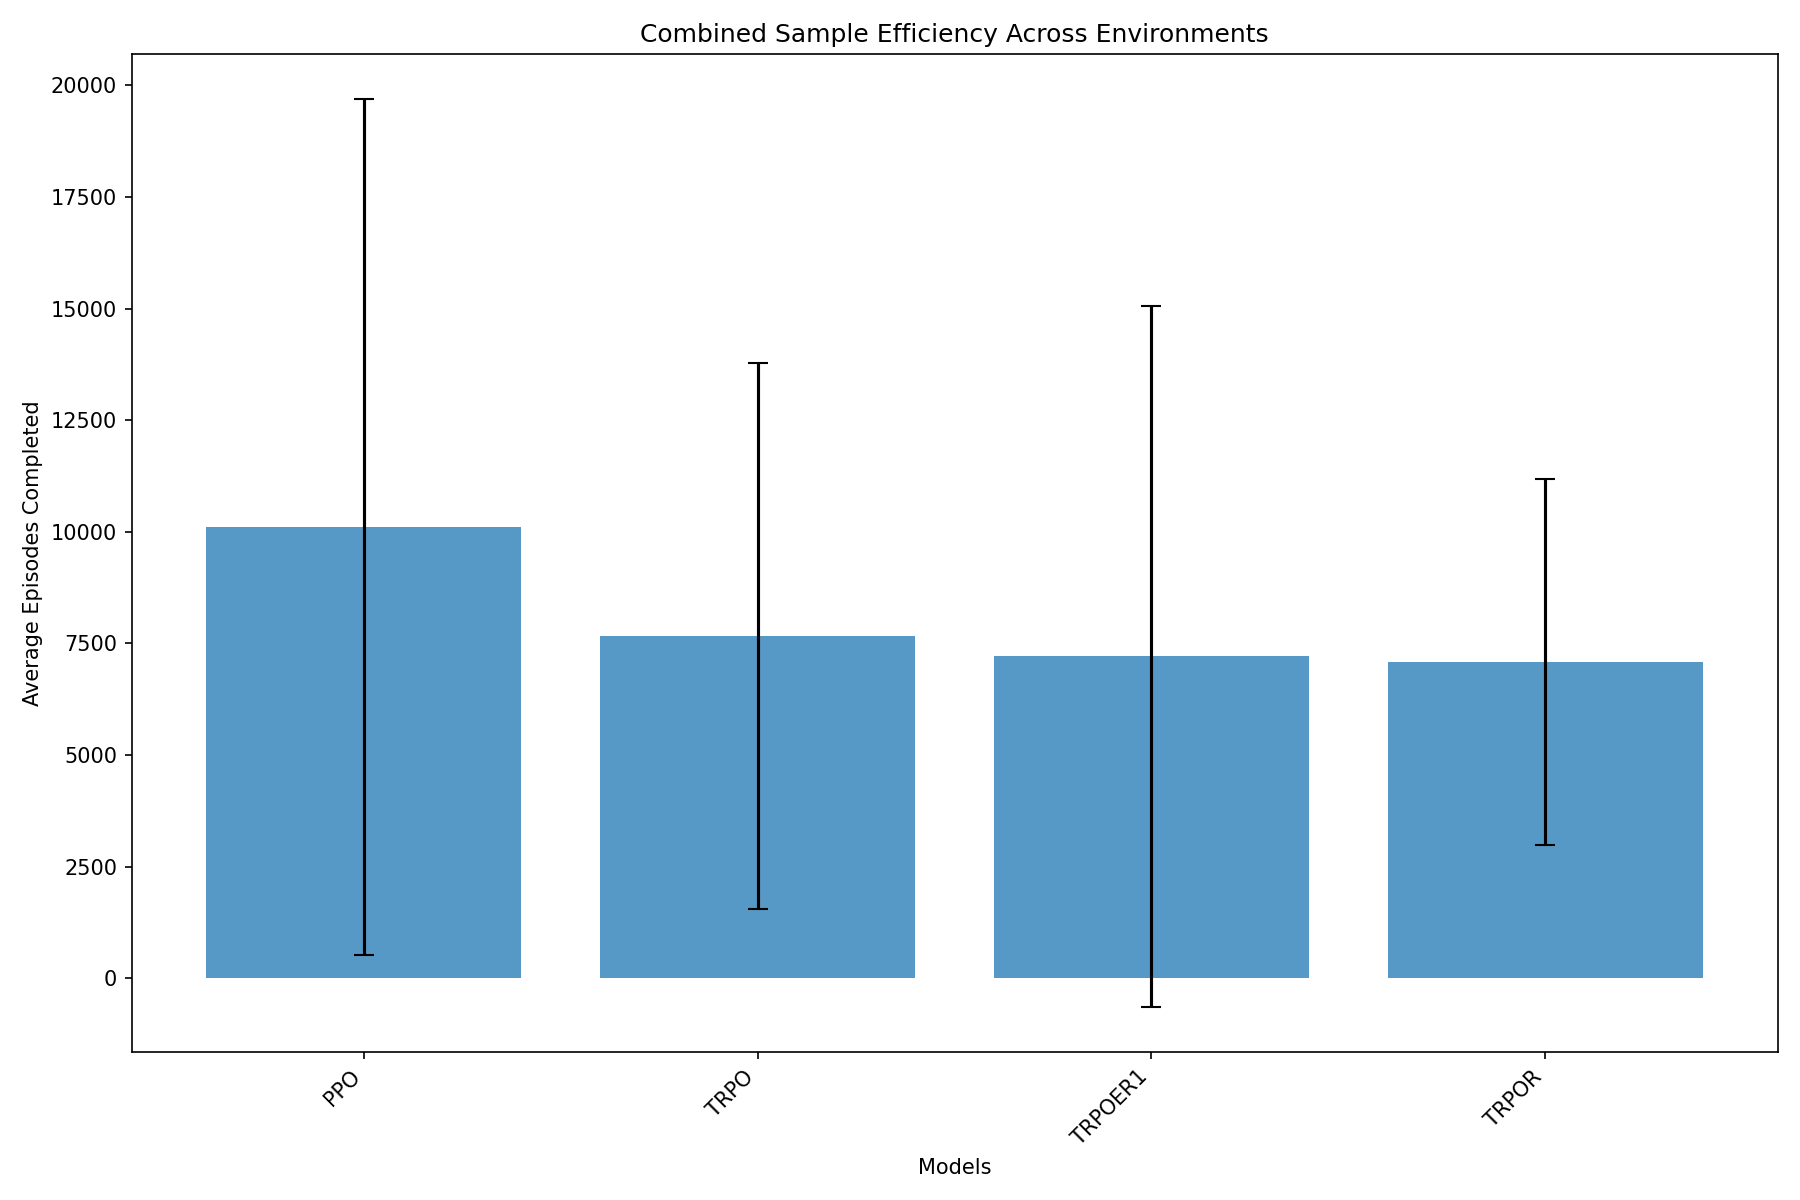
\includegraphics[width=0.8\textwidth]{.assets/sample_efficiency_combined.png}
    \caption{Combined Sample Efficiency Results}
\end{figure}

The combined sample efficiency plot aggregates results across all environments, showing how different models perform in terms of data efficiency.

\subsection{Raw Data}

\begin{figure}[H]
    \centering
    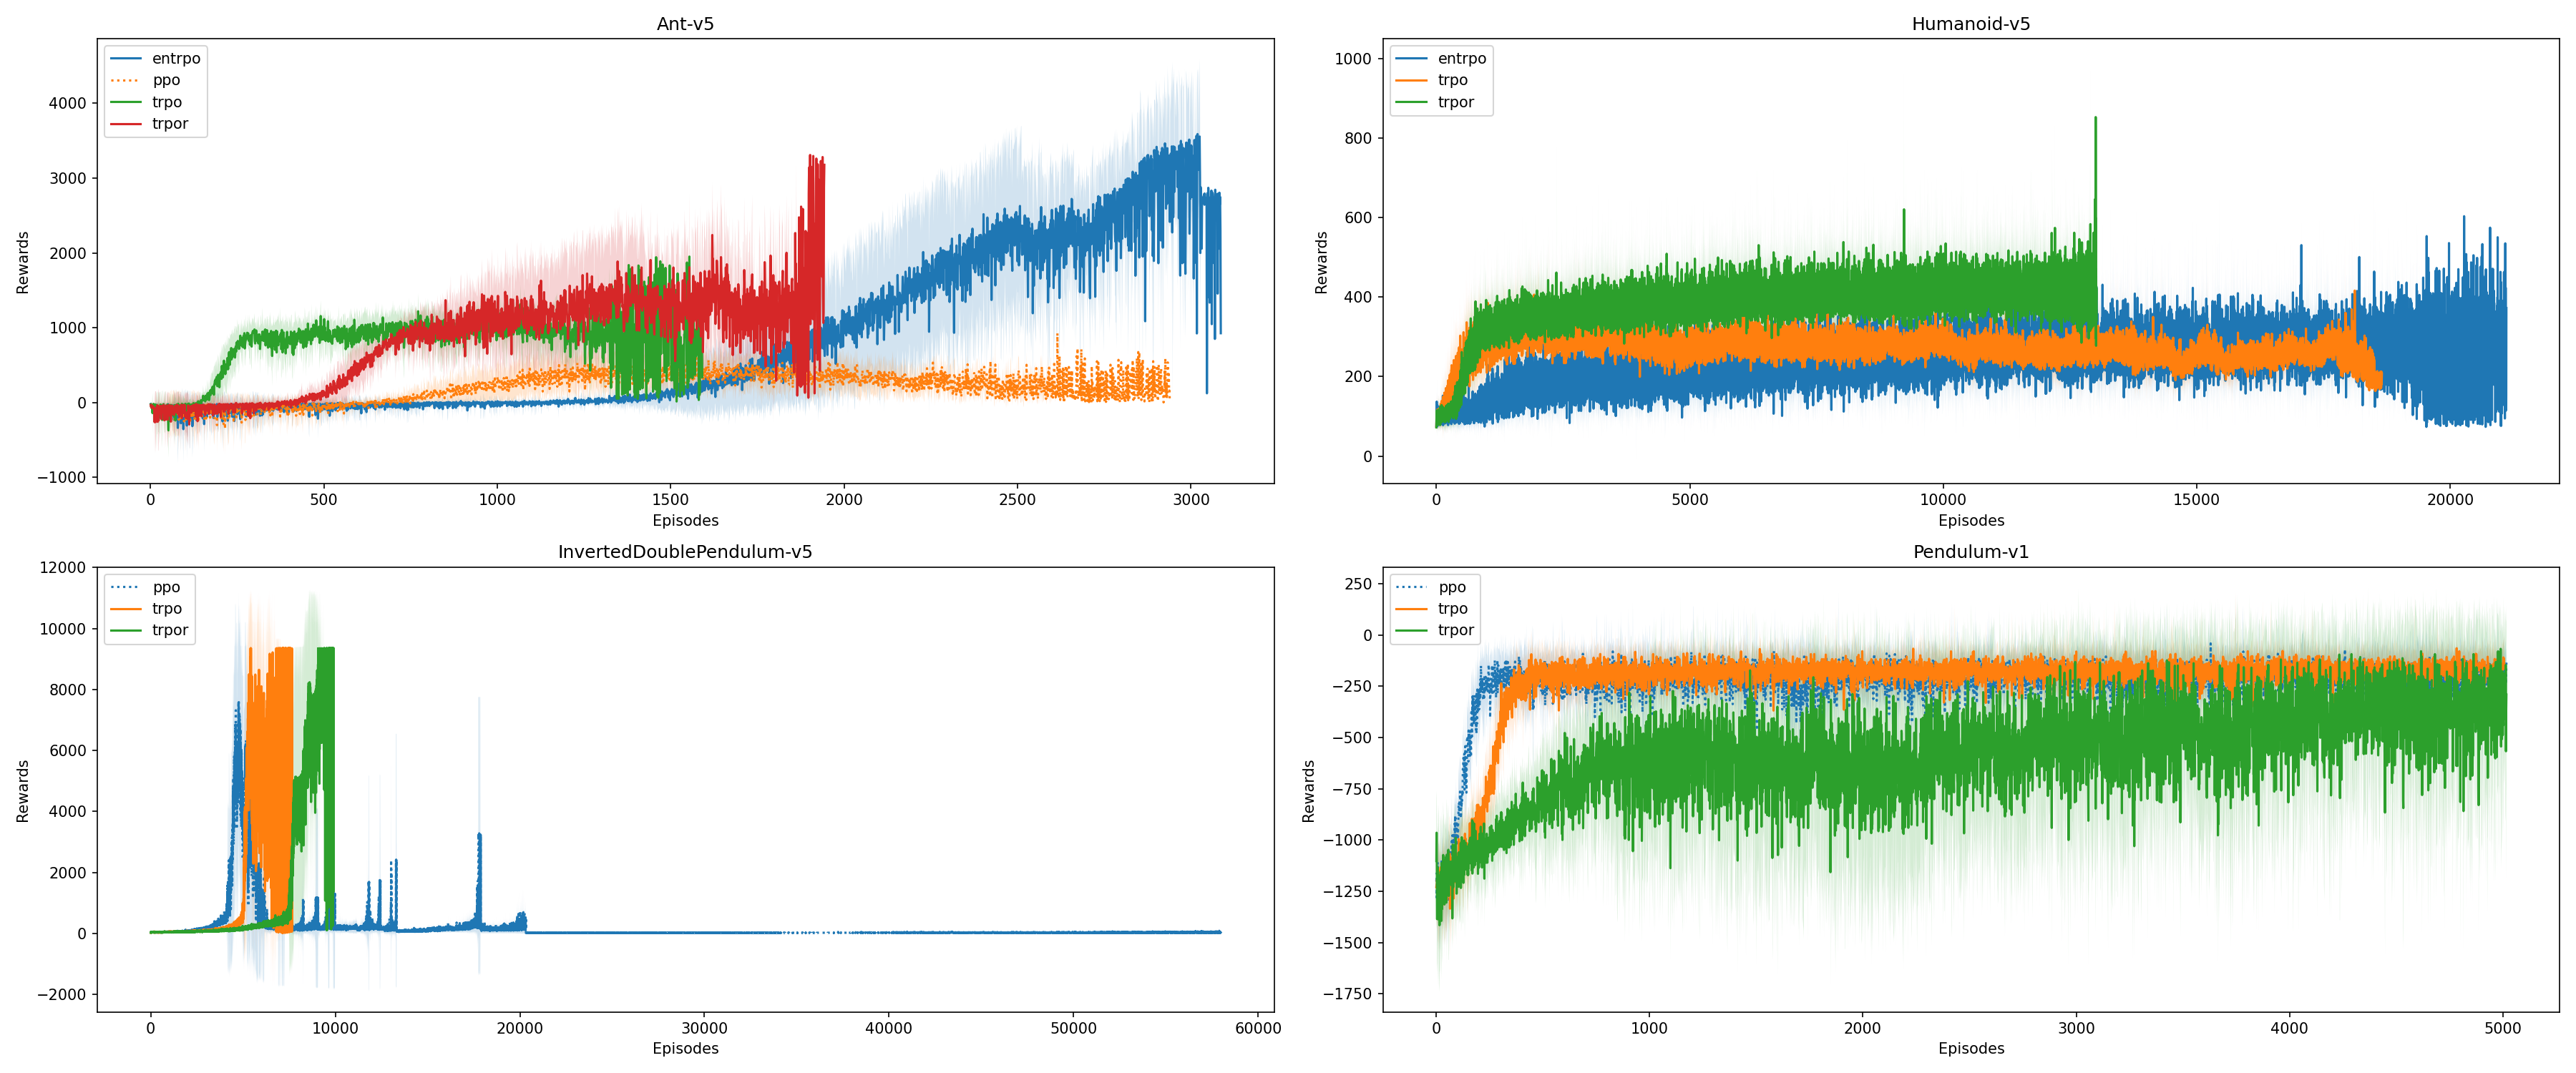
\includegraphics[width=0.8\textwidth]{.assets/raw_data.png}
    \caption{Raw Reward Data for Different Models}
\end{figure}

The raw data plot displays the recorded reward values without any smoothing. It provides insights into the actual training process and variability in rewards.


%----------------------------------------------------------

\section{Noise Injection Experimentation}
We conducted a series of experiments to evaluate the impact of noise injection on model performance. The goal was to assess how noise affects exploration and robustness in continuous control tasks. Our methodology involved injecting uniform noise into actions and rewards, varying the noise magnitude across different configurations. We detail methodology, results, and analysis below.

\subsection{Noise Injection Methodology}

Exploration remains a persistent challenge in reinforcement learning (RL), particularly in continuous action spaces where conventional methods such as $\epsilon$-greedy or Gaussian action noise often fall short in adequately sampling the environment \cite{plappert2018parameterspacenoiseexploration}. Recent research has shown that injecting noise into various RL components—such as actions, rewards, or model parameters—can enhance exploration and bolster robustness \cite{plappert2018parameterspacenoiseexploration, wang2020reinforcementlearningperturbedrewards}. Given that the models under evaluation (GenTRPO, TRPOER, and TRPOR) are entropy-regularized variants of TRPO \cite{schulman2017trustregionpolicyoptimization}, we hypothesize that introducing noise into the environment’s actions or rewards can amplify the exploratory behavior guided by entropy regularization, thereby improving both performance and robustness in continuous control tasks.

Our methodology employs a controlled noise injection framework utilizing a uniform distribution, selected for its bounded and symmetric properties. This choice aligns with the bounded action spaces typical of continuous control environments and ensures perturbations remain manageable, unlike the unbounded nature of Gaussian noise. We explored various noise distributions—Gaussian, Bernoulli, and uniform—targeting actions, rewards, and observations. Empirical trials revealed that uniform noise applied to actions and rewards, within the range $[-0.5, 0.5]$, produced the most consistent and significant improvements across all models. Noise on observations showed less universal benefit and is thus excluded from our primary analysis.

\subsection{Uniform Noise Model}
For a uniform random variable $X \sim \text{Uniform}(a, b)$, the probability density function is:
\begin{equation}
f(x) = 
\begin{cases} 
\frac{1}{b - a}, & a \leq x \leq b, \\
0, & \text{otherwise},
\end{cases}
\end{equation}
with mean $\mathbf{E}[X] = \frac{a + b}{2}$ and variance $\text{Var}(X) = \frac{(b - a)^2}{12}$. By setting $a = -b$, we ensure zero-mean noise, preventing systematic bias in the perturbed signals.

\subsection{Action Noise Injection}
Action noise perturbs the agent’s control outputs to simulate environmental variability or motor inaccuracies, fostering exploration. For an action vector $a \in \mathbf{R}^n$, where $n$ is the action space dimensionality, the noisy action $a'$ is defined as:
\begin{equation}
a' = a + \eta_a, \quad \eta_a \sim \text{Uniform}(-\epsilon_a \cdot R_{\text{base}}, \epsilon_a \cdot R_{\text{base}})^n,
\end{equation}
where $\epsilon_a \in [0, 1]$ is a scaling factor controlling noise magnitude, and $R_{\text{base}} = 1.0$ is a constant range. The variance per component is:
\begin{equation}
\text{Var}(\eta_{a,i}) = \frac{\epsilon_a^2}{3}.
\end{equation}
The perturbed action is constrained to the environment’s bounds via clipping:
\begin{equation}
a_{\text{used}} = \text{clip}(a', a_{\text{low}}, a_{\text{high}}),
\end{equation}
ensuring feasibility. This approach differs from parameter noise \cite{plappert2018parameterspacenoiseexploration}, which targets policy weights, offering a direct, environment-level exploration mechanism.

\subsection{Reward Noise Injection}
Reward noise introduces uncertainty into the feedback signal, testing robustness against real-world variability \cite{wang2020reinforcementlearningperturbedrewards}. For a scalar reward $r$, the noisy reward $r'$ is:
\begin{equation}
r' = r + \eta_r, \quad \eta_r \sim \text{Uniform}(-\epsilon_r \cdot R_{\text{base}}, \epsilon_r \cdot R_{\text{base}}),
\end{equation}
with variance $\text{Var}(\eta_r) = \frac{\epsilon_r^2}{3}$. Unlike actions, rewards are not clipped, allowing the full perturbation range to influence learning dynamics.

%-----------------------------------------------------------

\subsection{Results and Analysis}

The following subsections present results for each model, comparing mean rewards and policy entropy under noise-injected conditions (\(\epsilon \in \{-0.5, -0.3, -0.1, 0.1, 0.3, 0.5\}\)) against a no-noise baseline to validate our hypotheses. Preliminary findings confirm that noise injection enhances exploration and robustness: entropy guides models toward broader or more efficient exploration, consistently improving performance over the baseline. Entropy-regularized models exhibit superior tolerance to perturbations in continuous action spaces, often surpassing baseline performance under identical conditions. Detailed analyses and visualizations follow.

\subsection{PPO}

We trained the PPO algorithm for 100,000 steps with action and reward noise injection, adhering to the standard formulation \cite{schulman2017proximalpolicyoptimizationalgorithms}. All six noise configurations and the baseline used identical hyperparameters, with five independent runs per configuration for statistical significance. Results show that noise injection reduces policy entropy in certain cases, enhancing exploration and leading to performance gains over the baseline, even when entropy exceeds baseline levels, as depicted in the figure below.

\vspace*{-\baselineskip}
\begin{figure}[H]
    \centering
    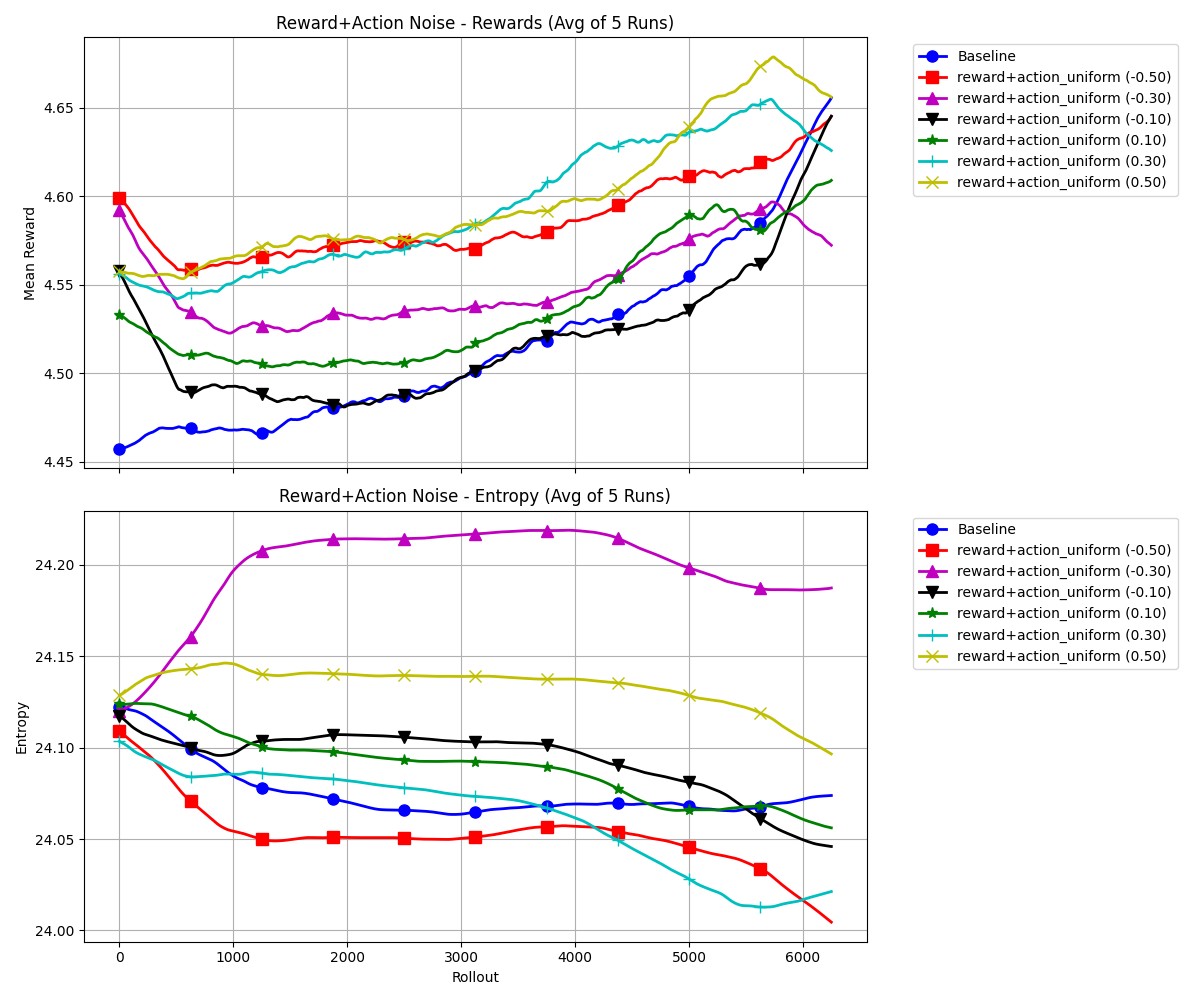
\includegraphics[width=0.8\textwidth]{.assets/PPO_100000_reward_action_5_runs_resmoothed.png}
    \caption{Performance of PPO with Action and Reward Noise Injection}
\end{figure}
\vspace*{-\baselineskip}

\subsection{TRPO}

Trust Region Policy Optimization (TRPO), a reference model, demonstrates greater tolerance to noise injection than PPO. Minibatch entropy increases across configurations, reflecting enhanced exploration. However, this does not always correlate with reward improvements: \(\epsilon = -0.5\) yields the lowest rewards, while \(\epsilon = 0.3\) achieves the highest, maintaining entropy akin to the baseline. This suggests an optimal noise level beyond which benefits diminish, as shown below.

\vspace*{-\baselineskip}
\begin{figure}[H]
    \centering
    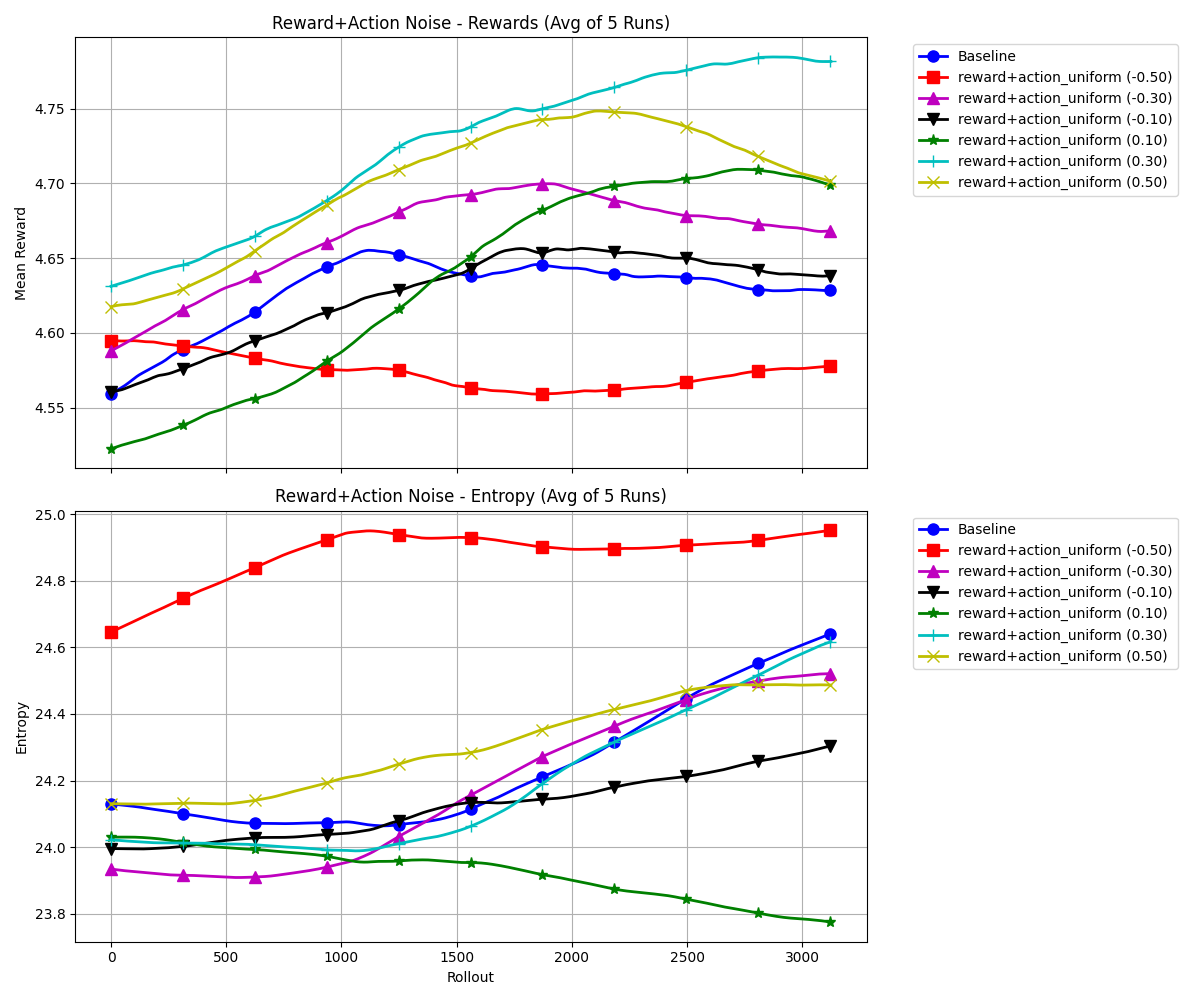
\includegraphics[width=0.8\textwidth]{.assets/TRPO_100000_reward_action_5_runs_resmoothed.png}
    \caption{Performance of TRPO with Action and Reward Noise Injection}
\end{figure}
\vspace*{-\baselineskip}

\subsection{GenTRPO}

GenTRPO exhibits exceptional behavior, with entropy decreasing logarithmically across all configurations while maintaining a consistent, tightly grouped curve. This robustness to perturbations enables entropy reduction despite regularization, with \(\epsilon = -0.1\) optimizing rewards within the empirical bounds \([-0.5, 0.5]\). Negative configurations (\(\epsilon = -0.5, -0.3, -0.1\)) outperform the baseline, while positive ones underperform, as illustrated below.

\vspace*{-\baselineskip}
\begin{figure}[H]
    \centering
    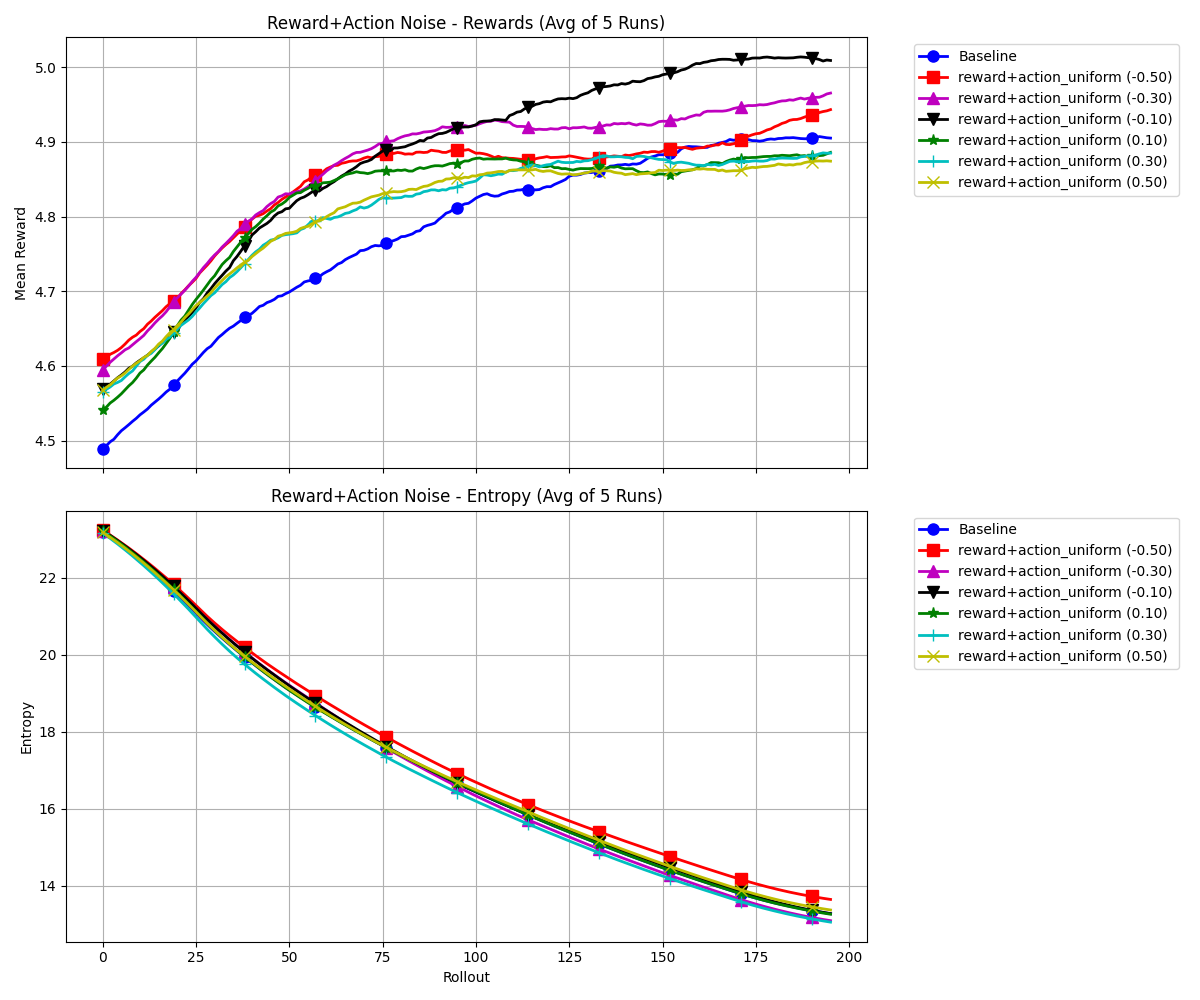
\includegraphics[width=0.8\textwidth]{.assets/GenTRPO_100000_reward_action_5_runs.png}
    \caption{Performance of GenTRPO with Action and Reward Noise Injection}
\end{figure}
\vspace*{-\baselineskip}

\subsection{TRPOR}

TRPOR, an entropy-regularized TRPO variant, mirrors GenTRPO’s entropy reduction across configurations, quickly surpassing its baseline. The \(\epsilon = -0.5\) configuration achieves the highest rewards, with approximately a 40\% improvement over the baseline, highlighting its ability to leverage noise for both exploration efficiency and robustness, as shown below.

\vspace*{-\baselineskip}
\begin{figure}[H]
    \centering
    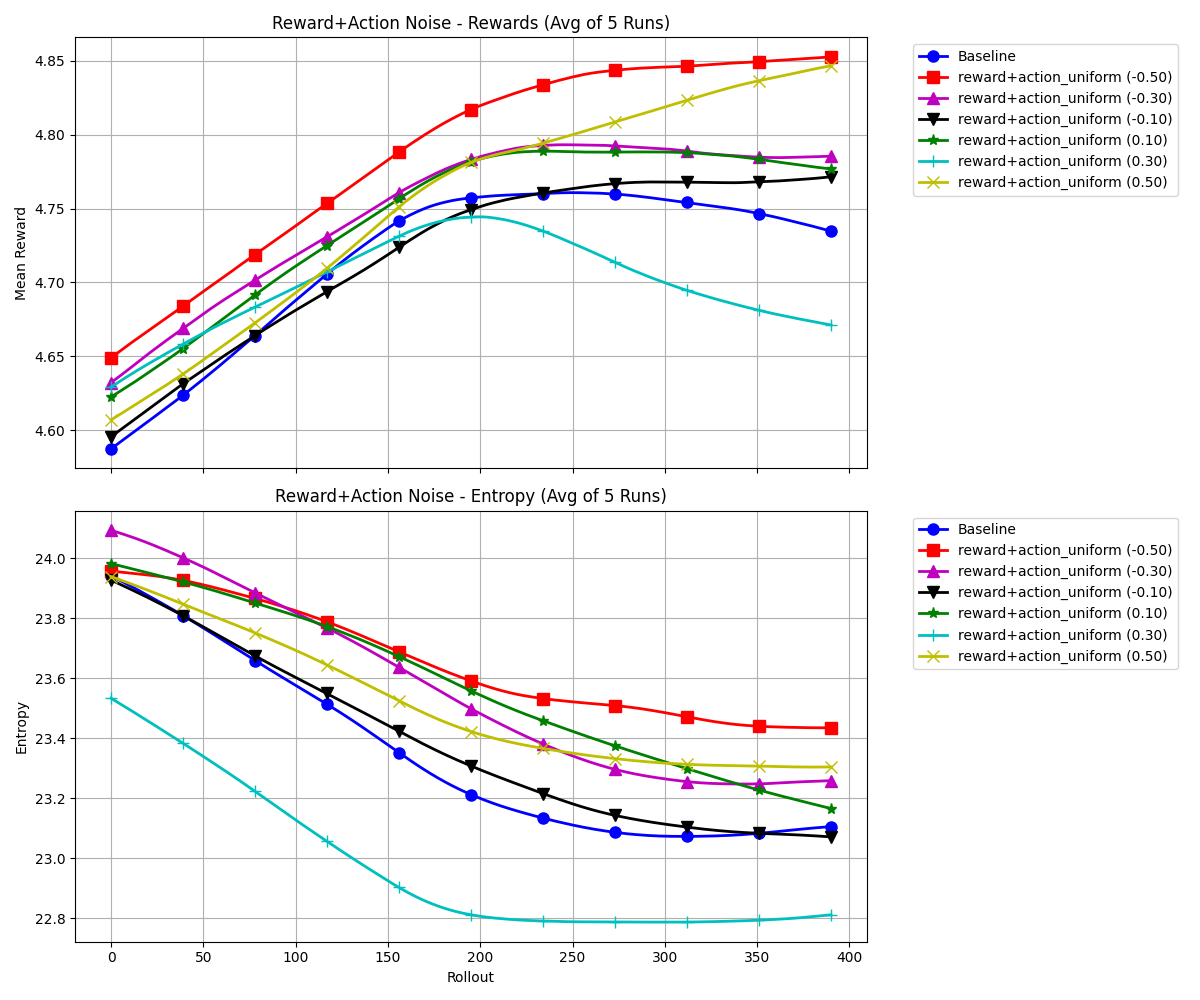
\includegraphics[width=0.8\textwidth]{.assets/TRPOR_100000_reward_action_5_runs_resmoothed.png}
    \caption{Performance of TRPOR with Action and Reward Noise Injection}
\end{figure}
\vspace*{-\baselineskip}

\subsection{TRPOER}

TRPOER, shows increasing entropy across all configurations, clustering into positive and negative groups. While no single optimal configuration emerges, noise injection consistently boosts rewards above the baseline, indicating enhanced exploration and robustness, as visualized below.

\vspace*{-\baselineskip}
\begin{figure}[H]
    \centering
    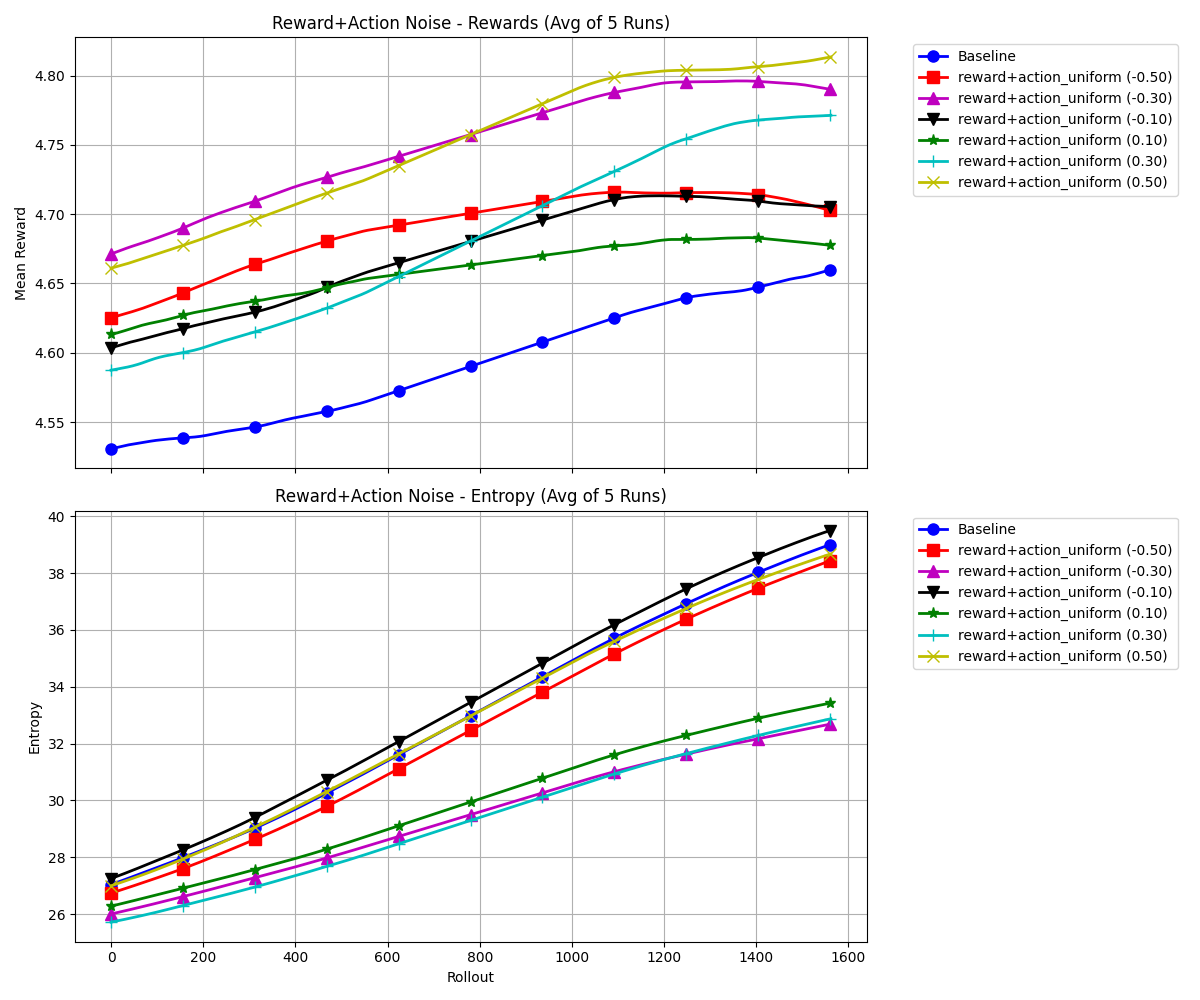
\includegraphics[width=0.8\textwidth]{.assets/TRPOER_100000_reward_action_5_runs_resmoothed.png}
    \caption{Performance of TRPOER with Action and Reward Noise Injection}
\end{figure}
\vspace*{-\baselineskip}

\subsection{Conclusion on Noise Injection}

Our results validate both hypotheses. The exploration hypothesis is confirmed: action noise enhances exploration, either by increasing entropy (TRPOR, TRPO) to broaden the policy search or by managing it efficiently within regularized frameworks (GenTRPO, TRPOER) to optimize performance, consistently surpassing baselines. The robustness hypothesis holds as well: reward noise improves tolerance to perturbations, with entropy-regularized models (GenTRPO, TRPOR, TRPOER) outperforming PPO and TRPO across all cases, leveraging adaptive mechanisms for superior reward gains. Optimal noise levels vary (\(\epsilon = -0.5\) for TRPOER, \(\epsilon = 0.3\) for TRPO), but benefits plateau beyond model-specific thresholds, reinforcing the efficacy of noise injection in enhancing exploration and robustness in continuous action spaces.

%----------------------------------------------------------




%----------------------------------------------------------

\newpage

\bibliographystyle{plain}
\bibliography{references}

\end{document}
